% \begin{lstlisting}
% 底层实现原理

% 不同硬件上的针对性加速:
% 1. avx
% 2. arm
% 3. 鲲鹏
% 4. GPU
% \end{lstlisting}
\subsection{State Vector Simulator}
\label{sec_state_vec}
\subsubsection{Policy Based Design pattern}
In \MindQuantum, we use \Simulator to simulate quantum state. A \Simulator maintain a quantum state, as mentioned in section \ref{sec:sim_basic_usage}, methods start with `apply' will change this maintained quantum state, and methods start with `get' will not change anything but only extrude information from the quantum state.

Simulating quantum systems imposes high performance requirements on simulators. In \MindQuantum, we utilize C++ or CUDA as the underlying simulator implementation language, accelerating quantum simulations based on different hardware instruction sets. We adopt a policy-based development approach, optimizing the fundamental simulator interface for different instruction sets and encapsulating them into policy types. Building upon a unified quantum simulation framework, we generate different quantum simulators using various simulator policies, such as AVX-supported simulators, neon-supported simulators, and GPU-supported simulators.

\begin{figure}[ht]
    \centering
    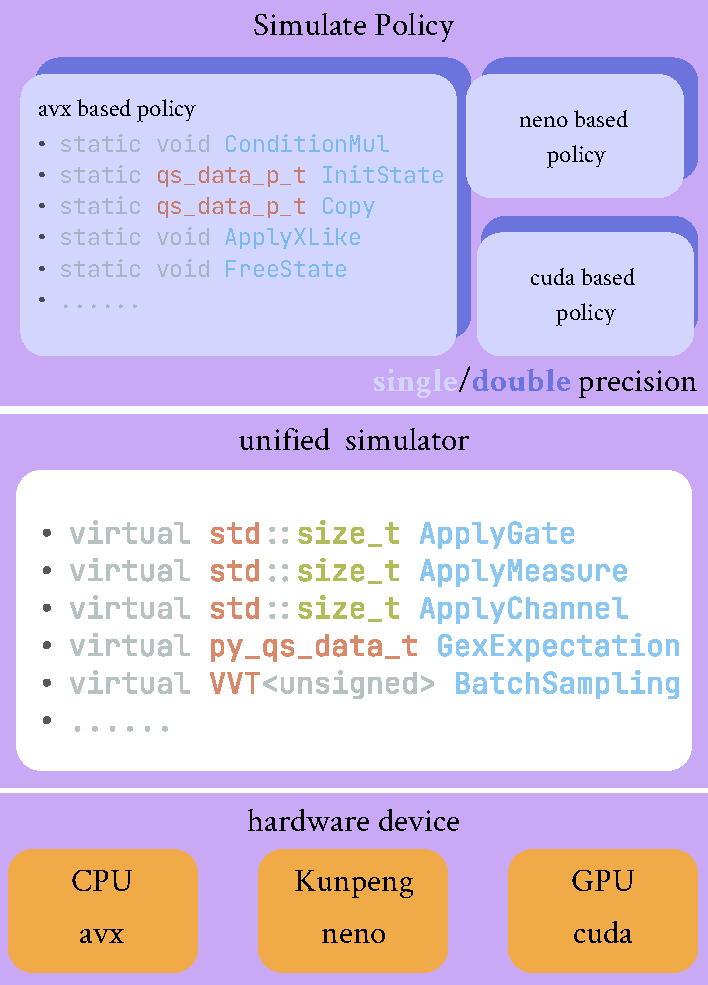
\includegraphics[scale=0.6]{./images/4_1_simulator_structure.pdf}
    \captionsetup{justification=raggedright,singlelinecheck=false}
    \caption{\label{4_1_sim_str} The layer structure of simulator in. The simulate policy layer applies quantum gate to quantum state based on actual simulation hardware. The unified simulator layer use different policy to finish circuit simulation and expectation and gradient calculation. The hardware device layer shows we support CPU, GPU and Kunpeng platform.}
\end{figure}

Depending on the specific quantum system being simulated, we have the option to choose between a full amplitude quantum simulator or a density matrix simulator. In \MindQuantum, these two simulators are referred to as `mqvector' and `mqmatrix', respectively. In the current \version version, the `mqvector' simulator also supports GPU acceleration and is named `mqvector\_gpu'. Both `mqvector' and `mqmatrix' use same design pattern in Fig.~\ref{4_1_sim_str}. Based on these simulators, noise simulation is also supported with the help of quantum channel, which will talked in section ~\ref{sec:noise_simulation}.

\subsubsection{Gate optimization with SIMD}
SIMD (Single Instruction Multiple Data) is a computer architecture and parallel processing technique designed to accelerate the execution of tasks that can be parallelized by applying a single operation to multiple data elements simultaneously. The fundamental building block of a quantum simulator is the interaction between quantum gate and quantum state, involving multiple parallel operations, so We can utilize SIMD to accelerate the speed of quantum simulations. In this section, we will show how to optimize gate evolution based on avx instruction with complex128 data type.

AVX instruction provide us a 256 bits width vector register, which can storage 4 numbers with double precision or two complex numbers with double precision. In Fig~\ref{fig:avx}, we take a two qubits full state vector for example, probability amplitude $a$ and $b$ can load to a 256 bits register simultaneously, and $c$ and $d$ the same.
\begin{figure}
    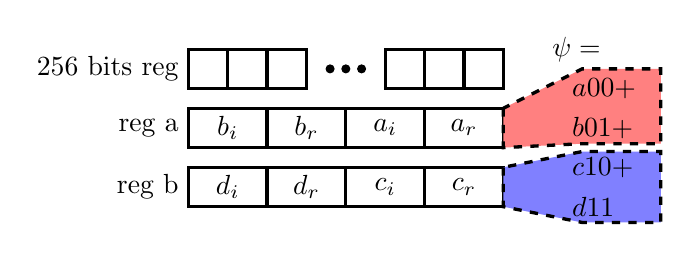
\begin{tikzpicture}[scale=0.5]
        \node[left] at (0,0.5) {256 bits reg};
        \draw[line width=1.2] (0,0) rectangle (1, 1);
        \draw[line width=1.2] (1,0) rectangle (2, 1);
        \draw[line width=1.2] (2,0) rectangle (3, 1);
        \draw[fill=black] (3.6, 0.5) circle (0.1);
        \draw[fill=black] (4.0, 0.5) circle (0.1);
        \draw[fill=black] (4.4, 0.5) circle (0.1);
        \draw[line width=1.2] (5,0) rectangle (6, 1);
        \draw[line width=1.2] (6,0) rectangle (7, 1);
        \draw[line width=1.2] (7,0) rectangle (8, 1);
        \node[left] at (0,-1) {reg a};
        \draw[line width=1.2] (0,-1.5) rectangle (2, -0.5);
        \draw[line width=1.2] (2,-1.5) rectangle (4, -0.5);
        \draw[line width=1.2] (4,-1.5) rectangle (6, -0.5);
        \draw[line width=1.2] (6,-1.5) rectangle (8, -0.5);
        \node at (1,-1) {$b_i$};
        \node at (3,-1) {$b_r$};
        \node at (5,-1) {$a_i$};
        \node at (7,-1) {$a_r$};
        \node[left] at (0,-2.5) {reg b};
        \draw[line width=1.2] (0,-3) rectangle (2, -2);
        \draw[line width=1.2] (2,-3) rectangle (4, -2);
        \draw[line width=1.2] (4,-3) rectangle (6, -2);
        \draw[line width=1.2] (6,-3) rectangle (8, -2);
        \node at (1,-2.5) {$d_i$};
        \node at (3,-2.5) {$d_r$};
        \node at (5,-2.5) {$c_i$};
        \node at (7,-2.5) {$c_r$};
        \draw[dashed, line width=1.2, fill=red!50] (8, -0.5) -- (8, -1.5) -- (10, -1.4) -- (12, -1.4) -- (12, 0.5) -- (10, 0.5) -- cycle;
        \draw[dashed, line width=1.2, fill=blue!50] (8, -2) -- (8, -3) -- (10, -3.4) -- (12, -3.4) -- (12, -1.6) -- (10, -1.6) -- cycle;
        \node[right] at (9, 1) {$\ket{\psi}=$};
        \node[right] at (9.5, -0) {$a\ket{00}+$};
        \node[right] at (9.5, -1) {$b\ket{01}+$};
        \node[right] at (9.5, -2) {$c\ket{10}+$};
        \node[right] at (9.5, -3) {$d\ket{11}$};
    \end{tikzpicture}
    \caption{Storage a 2 qubits quantum state into two 256 bits registers.}
    \label{fig:avx}
\end{figure}

We split basic quantum gate into different type, such X-like, Z-like or matrix gate. For X-like gate, the elements are only in anti-diagonal:
\begin{equation}
    \begin{pmatrix}
        0 & a \\
        b & 0
    \end{pmatrix}.
\end{equation}
When X-like gate is act on first qubit, we need to swap $(b*a_r, b*a_i)$ and $(a*b_r, a*b_i)$ in a single avx register. And if this gate is act on other qubit, then we need to swap $b*\text{reg\_a}$ and $a*\text{reg\_b}$. For Z-like gate, the elements are only in diagonal:
\begin{equation}
    \begin{pmatrix}
        a & 0 \\
        0 & b
    \end{pmatrix}
\end{equation}
In this situation, we just need to change $(a_r, a_i)$ to $(a*a_r, a*a_i)$ and $(b_r, b_i)$ to $(b*b_r, b*b_i)$ if the gate act on first qubit, or just multiply $a$ to reg a and multiply $b$ to reg b if acting on other qubit.

\subsection{Density Matrix Simulator}
Different from state vector simulator, density matrix simulator is more suitable for mix state or open quantum system simulation, but much more memory consuming. The density operator of a quantum system is described as:
\begin{equation}
    \rho=\sum_ip_i\ket{\psi_i}\bra{\psi_i},
\end{equation}
where $p_i$ is the probability of system in pure state $\ket{\psi_i}$. The evolution of a quantum gate $U$ on density operator is:
\begin{equation}
    \rho'=U\rho U^\dagger.
\end{equation}
The expectation of a observable $H$ under $\rho$ is:
\begin{equation}
    \left<H\right> = \sum_ip_i\bra{\psi_i}H\ket{\psi_i}=\tr(\rho H)
\end{equation}.

The usage, developing strategy and optimization process is very similar with state vector simulator, please refers to section ~\ref{sec_state_vec}.
